%%%%%%%%%%%%%%%%%%%%%%%%%%%%%%%%%%%%%%%%%%%%%%%%%%%%%%%%%
%%%  浮点数对象
%%%%%%%%%%%%%%%%%%%%%%%%%%%%%%%%%%%%%%%%%%%%%%%%%%%%%%%%%
\chapter{Python 浮点数对象}

本章要研究的主题是 Python 中的浮点数对象。

\section{inf、-inf 与 nan}
为了方便理解之后讲解代码中的一些实现,简单介绍一下 inf,-inf,nan 三个概念。
\begin{itemize}
\item inf: 正无穷大
\item -inf:负无穷小
\item nan: not a number 非数字
\end{itemize}

下面使用 Python 解释器进行一些简单的测试。

\begin{lstlisting}[language=Python, numbers=left, numbersep=1em, numberstyle=\footnotesize , breaklines=true]
>>> inf = float('inf')
>>> ninf = float('-inf')
>>> nan = float('nan')
>>> inf > ninf
True
>>> inf > nan
False
>>> ninf > nan
False
>>> -100 > ninf
True
>>> 100 < inf
True
>>> inf + ninf
nan
>>> inf + 0
inf
>>> inf + 1
inf
>>> inf + nan
nan
\end{lstlisting}

由于涉及这三个概念的运算规则不在我们的介绍范围之内,所以这里不做讲解。这三个概念都是由
IEEE 754 规范所定义,主要是用来处理针对浮点数的极端情况。下面是引用的一段 IEEE 754 中对所有浮点数的定义,感兴趣的
读者可以从本章的参考资料给出的链接去阅读 IEEE 754 规范原文。

IEEE 754 encodes floating-point numbers in memory (not in registers) in ways first proposed by I.B. Goldberg
in Comm. ACM (1967) 105-6 ; it packs three fields with integers derived from the sign, exponent and significand
of a number as follows. The leading bit is the sign bit, 0 for + and 1 for - . The next K+1 bits hold a biased
exponent. The last N or N-1 bits hold the significand's magnitude. To simplify the following table, the
significand n is dissociated from its sign bit so that n may be treated as nonnegative.

\begin{figure}[htbp]
\centering
  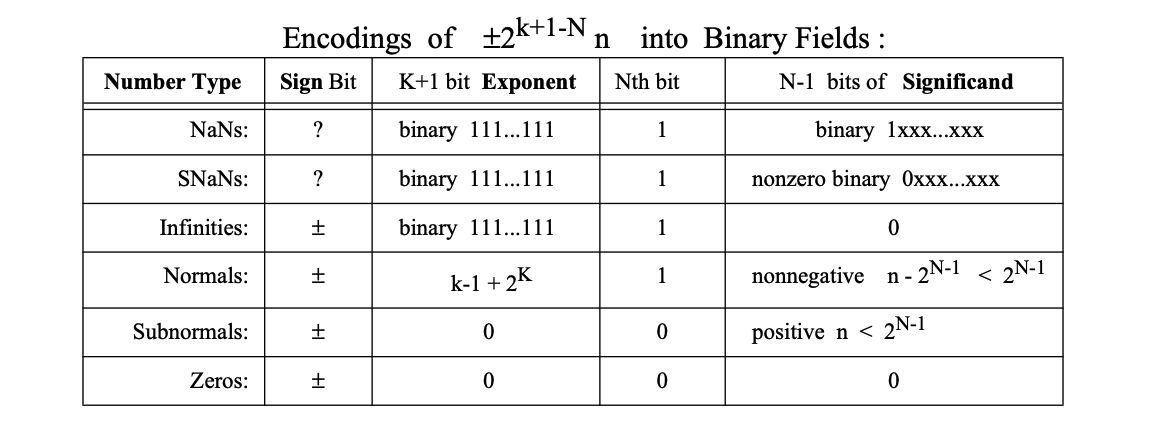
\includegraphics[width=1.0\textwidth]{pictures/inf_and_nan.png}
  \caption{IEEE754 float 定义 \label{fig:scatter}}
\end{figure}

\section{PyFloatObject}

\begin{lstlisting}[language=C, numbers=left, numbersep=1em, numberstyle=\footnotesize , breaklines=true]
// Include/floatobject.h
typedef struct {
    PyObject_HEAD
    double ob_fval;
} PyFloatObject;
\end{lstlisting}

PyFloatObject 对象的定义如上,PyObject\_HEAD 字段是大小不可变的 Python object 的统一头部,
ob\_fval 字段则是存储的 float 对象实际的值。为什么可以肯定的说 ob\_fval 存储的值就是 float 对象实际的值呢? 
我们可以通过一个实验来证明。在 Python 中可以通过下面的代码可以创建一个 float 对象,也就是虚拟机中的一个 PyFloatObject 对象。

\begin{lstlisting}[language=bash, numbers=left, numbersep=1em, numberstyle=\footnotesize , breaklines=true]
>>> f = float(3.14)
\end{lstlisting}

通过跟踪堆栈,发现最后进入了如下 PyFloat\_FromDouble 这个创建 PyFloatObject 对象的函数,在这个函数中,double 类型的
数字 3.14 被赋值给了 ob\_fval。

\begin{lstlisting}[language=C, numbers=left, numbersep=1em, numberstyle=\footnotesize , breaklines=true]
// Objects/floatobject.c
PyObject *
PyFloat_FromDouble(double fval)
{
    struct _Py_float_state *state = get_float_state();
    PyFloatObject *op = state->free_list;
    if (op != NULL) {
#ifdef Py_DEBUG
        // PyFloat_FromDouble() must not be called after _PyFloat_Fini()
        assert(state->numfree != -1);
#endif
        state->free_list = (PyFloatObject *) Py_TYPE(op);
        state->numfree--;
    }
    else {
        op = PyObject_Malloc(sizeof(PyFloatObject));
        if (!op) {
            return PyErr_NoMemory();
        }
    }
    _PyObject_Init((PyObject*)op, &PyFloat_Type);
    // 通过单步调试,发现最后 3.14 被赋值给了 op->ob_fval
    // 由此我们断定 ob_fval 被用来保存浮点数对象的真实值
    op->ob_fval = fval;
    return (PyObject *) op;
}
\end{lstlisting}

\section{对象池机制}

Python 的内置对象属于使用的非常频繁的对象,为了避免频繁的创建和释放这些类型的对象,Python 为他们设计
了一个对象池的机制。以本章研究的 PyFloatObjet 对象为例,我们来研究一下 Python 是如何实现它的对象池机制的。
首先看一下 PyFloatObject 在什么时候会使用对象池。

\begin{lstlisting}[language=C, numbers=left, numbersep=1em, numberstyle=\footnotesize , breaklines=true]
// Objects/floatobject.c
PyObject *
PyFloat_FromDouble(double fval)
{
    struct _Py_float_state *state = get_float_state();
    // [1] 获取对象池中的元素
    PyFloatObject *op = state->free_list;
    if (op != NULL) {
#ifdef Py_DEBUG
        // PyFloat_FromDouble() must not be called after _PyFloat_Fini()
        assert(state->numfree != -1);
#endif
	  // [2] 如果从空闲链表中获取到了元素,则需要将获取到的元素的
	  // 类型转换为 PyFloatObject
        state->free_list = (PyFloatObject *) Py_TYPE(op);
        // [3] 空闲链表上的元素数量减少1
        state->numfree--;
    }
    else {
        // [4] 空闲链表上没有元素了,则按照正常流程进行申请内存分配
        op = PyObject_Malloc(sizeof(PyFloatObject));
        if (!op) {
            return PyErr_NoMemory();
        }
    }
    // [5] 对获取到的对象进行初始化
    _PyObject_Init((PyObject*)op, &PyFloat_Type);
    op->ob_fval = fval;
    return (PyObject *) op;
}

\end{lstlisting}

PyFloat\_FromDouble 函数中的 state->free\_list 就是我们说的对象池了(虽说是对象池,但是叫做空闲对象链表更加合适一点)。 
可以看到流程是先调用 get\_float\_state 函数获取 struct \_Py\_float\_state* 类型的指针指向的一个 \_Py\_float\_state 实例 state,再
获取 state 上的 free\_list 作为我们需要的 PyFloatObject 对象。可以在这里没有到把这个元素从链表中取出的操作,也没有看到明显的对
链表的维护代码,难道这个叫做 free\_list 的东西只含有一个元素吗,那它为什么被叫做 list 呢?别着急,通过下面的分析,我们马上就可以
知道这些问题的答案了。不过我们还是先回到上面的代码,看一下如果没有从空闲链表中拿到元素,要怎么处理。从代码中的 [4] 处可
以看到,如果空闲链表中没有空闲的元素了,那么会走一个正常的申请内存分配的流程。不管是从空闲链表获取到的元素,还是通过
内存分配获取到的元素,在 [5] 处都要进行  PyFloatObject 对象的初始化。初始化的细节稍后再分析,我们下面回到空闲链表的话题。

先看一下持有了 free\_list 的家伙 \_Py\_float\_state 是什么一个构造。

\begin{lstlisting}[language=C, numbers=left, numbersep=1em, numberstyle=\footnotesize , breaklines=true]
struct _Py_float_state {
    /* Special free list
       free_list is a singly-linked list of available PyFloatObjects,
       linked via abuse of their ob_type members. */
    int numfree;
    PyFloatObject *free_list;
};
\end{lstlisting}

它的实现非常之简单,一个 numfree 成员表示空闲链表上元素的数量。还有一个 free\_list 指针。这个指针就是串联空闲链表的元素吗,
为什么看不到我们一般实现链表时候的 prev,next 指针呢,在上面的分析中,PyFloatObject 对象上可不存在这两个家伙。答案就藏在代码
的注释中,free\_list 通过利用 PyFloatObject 的 ob\_type 成员来链接链表上的元素。看起来很不可以思议,但其实都在情理之中,首先
空闲链表上的元素不需要 ob\_type 成员来表明类型,所以 ob\_type 可以被用作其他目的,例如这里的把空闲元素串连起来。其次,如果
需要按照标准的做法,使用一个 next 指针保存空闲链表的下一个元素,就需要在实现中多添加一个指针的大小,仅仅为了这个目的就增加
PyFloatObject 的内存大小,明显是得不偿失的,PyFloatObject 对象这种在运行时会大量创建的简单对象,每一个成员的添加都需要精打细算,避免造成过多的内存占用。从这两点看,使用 ob\_type 来链接空闲对象就很合理了。

清楚了空闲链表是如何串连起来的,接着研究一下我们上面提出的问题:空闲链表上的元素是如何被取下来的?
回到函数 PyFloat\_FromDouble。

\begin{lstlisting}[language=C, numbers=left, numbersep=1em, numberstyle=\footnotesize , breaklines=true]
PyObject *
PyFloat_FromDouble(double fval)
{
   // ... ...
    if (op != NULL) {
	  // ... ...
	  // [1] free_list 在这里指向了空闲链表中的下一个元素
        state->free_list = (PyFloatObject *) Py_TYPE(op);
        state->numfree--;
    }
	// ... ...
}

#define _PyObject_CAST(op) ((PyObject*)(op))

// [2] 返回的是 ob->ob_type
#define Py_TYPE(ob)             (_PyObject_CAST(ob)->ob_type)
\end{lstlisting}

看到上面的代码是不是恍然大悟了?在 [1] 处 free\_list 其实被赋予了一个新的值,这个新的值就是 [2] 处返回的当前 free\_list 首
元素的 ob\_type,在空闲链表的语境下,ob\_type 代表的就是空闲链表首个元素的下一个元素!

% 此处分析一下元素是如何添加到空闲链表的
知道了元素如何从空闲链表上取下来,那么我们一定也想知道元素是如何被添加到空闲链表上的。要了解这一点,可以从观察
PyFloatObject 对象 是如何被释放入手。

\begin{lstlisting}[language=C, numbers=left, numbersep=1em, numberstyle=\footnotesize , breaklines=true]
// Objects/floatobject.c

#  define PyFloat_MAXFREELIST   100

static void
float_dealloc(PyFloatObject *op)
{
    if (PyFloat_CheckExact(op)) {
        struct _Py_float_state *state = get_float_state();
#ifdef Py_DEBUG
        // float_dealloc() must not be called after _PyFloat_Fini()
        assert(state->numfree != -1);
#endif
	  // [1] 空闲链表达到上限,元素直接释放
        if (state->numfree >= PyFloat_MAXFREELIST)  {
            PyObject_Free(op);
            return;
        }
        // [2] 空闲链表没有达到上限,元素添加到空闲链表
        state->numfree++;
        Py_SET_TYPE(op, (PyTypeObject *)state->free_list);
        // [3] 要释放的元素变成了新的空闲链表头节点
        state->free_list = op;
    }
    else {
        Py_TYPE(op)->tp_free((PyObject *)op);
    }
}

// Include/object.h

// [4] 实际上就是 op->ob_type == state->free_list
static inline void _Py_SET_TYPE(PyObject *ob, PyTypeObject *type) {
    ob->ob_type = type;
}
#define Py_SET_TYPE(ob, type) _Py_SET_TYPE(_PyObject_CAST(ob), type)
\end{lstlisting}

从 [1] 处知道,如果空闲链表中连接的空闲元素数量达到了上限(当前版本中上限被定义为 100),那么就会将待释放的
元素直接释放。如果没有达到上限,才会考虑添加到空闲链表中。 [2] 处代码中调用了 Py\_SET\_TYPE 宏,而这个宏的
两个参数恰恰就是要释放的元素和空闲链表的头节点。结合 [3]、 [4] 两处的代码我们知道了,空闲链表的头节点成了
要释放元素 op 的下一个节点,op 变成了新的空闲链表头节点。

% 此处分析一下空闲链表是被谁管理的

了解清楚了空闲链表的机制,现在考虑新的问题:空闲链表是被谁管理的?多线程环境中空闲链表是怎么处理的?
带着这些问题,我们继续研究代码。get\_float\_state 函数作为获取 state 的入口,看一下它的内部实现。

\begin{lstlisting}[language=C, numbers=left, numbersep=1em, numberstyle=\footnotesize , breaklines=true]
// Objects/floatobject.c
static struct _Py_float_state *
get_float_state(void)
{
    // [1] 获取当前线程的解释器状态
    PyInterpreterState *interp = _PyInterpreterState_GET();
    return &interp->float_state;
}

// Include/internal/pycore_pystate.h
/* Get the current interpreter state.
   The macro is unsafe: it does not check for error and it can return NULL.
   The caller must hold the GIL.
   See also _PyInterpreterState_Get()
   and _PyGILState_GetInterpreterStateUnsafe(). */
static inline PyInterpreterState* _PyInterpreterState_GET(void) {
	// [2] 可以看到,这个 tstate 是每个线程都有一个的
    PyThreadState *tstate = _PyThreadState_GET();
#ifdef Py_DEBUG
    _Py_EnsureTstateNotNULL(tstate);
#endif
    return tstate->interp;
}
\end{lstlisting}

在 [1] 处代码可以看出,我们获取的 state 其实是一个 PyInterpreterState 的指针。看一下 PyInterpreterState 的定义。

\begin{lstlisting}[language=C, numbers=left, numbersep=1em, numberstyle=\footnotesize , breaklines=true]
// Include/pystate.h
typedef struct _is PyInterpreterState;

// Include/internal/pycore_interp.h
struct _is {
	// ... ...
	
   // 小整数池
    PyLongObject* small_ints[_PY_NSMALLNEGINTS + _PY_NSMALLPOSINTS];
    struct _Py_bytes_state bytes;
    struct _Py_unicode_state unicode;
    // PyFloatObject 空闲链表管理器
    struct _Py_float_state float_state;
    /* Using a cache is very effective since typically only a single slice is
       created and then deleted again. */
    PySliceObject *slice_cache;

    struct _Py_tuple_state tuple;
    struct _Py_list_state list;
    struct _Py_dict_state dict_state;
    struct _Py_frame_state frame;
    struct _Py_async_gen_state async_gen;
    struct _Py_context_state context;
    struct _Py_exc_state exc_state;
   // ... ...
};
\end{lstlisting}

可以看到,PyInterpreterState 这个结构不仅含有一个 PyFloatObject 空闲链表管理器,对其他多种 Python 内置对象,如 tuple,dict,int 等
都设置有对应的缓存机制。并且 PyInterpreterState 表示进程对象,Python 通过这个结构来模拟一个操作系统的进程,Python 的每个进程对应一个 PyInterpreterState 结构体。现在可以回答第一个问题了,空闲链表是被 PyInterpreterState 管理的。

回到上面的代码中,在摘抄代码时,我们特意留下了\_PyInterpreterState\_GET 函数的注释,注释中说到这个函数是不安全的,调用者
在调用这个函数的时候必须持有 GIL。而我们知道,这个 GIL 就是Python 中排他性的一个锁,每个线程要运行,就必须获得这把锁,所以
在调用 \_PyInterpreterState\_GET 时,必定只有一个线程能访问 PyInterpreterState,也就是说,空闲链表不会同时被 2 个及以上的线程访问,这也就可以回答前面提出的第二个问题:Python 通过 GIL 避免了多个线程同时访问空闲链表。

\begin{definition}[Python 对 GIL 的解释] \label{def:int}
  Notes about the implementation:

   - The GIL is just a boolean variable (locked) whose access is protected
     by a mutex (gil\_mutex), and whose changes are signalled by a condition
     variable (gil\_cond). gil\_mutex is taken for short periods of time,
     and therefore mostly uncontended.

   - In the GIL-holding thread, the main loop (PyEval\_EvalFrameEx) must be
     able to release the GIL on demand by another thread. A volatile boolean
     variable (gil\_drop\_request) is used for that purpose, which is checked
     at every turn of the eval loop. That variable is set after a wait of
     `interval` microseconds on `gil\_cond` has timed out.

      [Actually, another volatile boolean variable (eval\_breaker) is used
       which ORs several conditions into one. Volatile booleans are
       sufficient as inter-thread signalling means since Python is run
       on cache-coherent architectures only.]

   - A thread wanting to take the GIL will first let pass a given amount of
     time (`interval` microseconds) before setting gil\_drop\_request. This
     encourages a defined switching period, but doesn't enforce it since
     opcodes can take an arbitrary time to execute.

     The `interval` value is available for the user to read and modify
     using the Python API `sys.{get,set}switchinterval()`.

   - When a thread releases the GIL and gil\_drop\_request is set, that thread
     ensures that another GIL-awaiting thread gets scheduled.
     It does so by waiting on a condition variable (switch\_cond) until
     the value of last\_holder is changed to something else than its
     own thread state pointer, indicating that another thread was able to
     take the GIL.

     This is meant to prohibit the latency-adverse behaviour on multi-core
     machines where one thread would speculatively release the GIL, but still
     run and end up being the first to re-acquire it, making the "timeslices"
     much longer than expected.
     (Note: this mechanism is enabled with FORCE\_SWITCHING above)
\end{definition}


\section{参考资料}

\begin{itemize}
\item \href{https://peps.python.org/pep-3101/}{PEP 3101 – Advanced String Formatting}
\item \href{http://li.mit.edu/Archive/Activities/Archive/CourseWork/Ju_Li/MITCourses/18.335/Doc/IEEE754/ieee754.pdf}{IEEE Standard 754 for Binary Floating-Point Arithmetic}
\end{itemize}


